%! Author = marcusdesai
%! Date = 28/08/2023

% Preamble
\documentclass[border=5pt]{standalone}

% Packages
\usepackage{amsmath}
\usepackage{tikz}
\usetikzlibrary{automata, positioning, arrows}

% Document
\begin{document}

    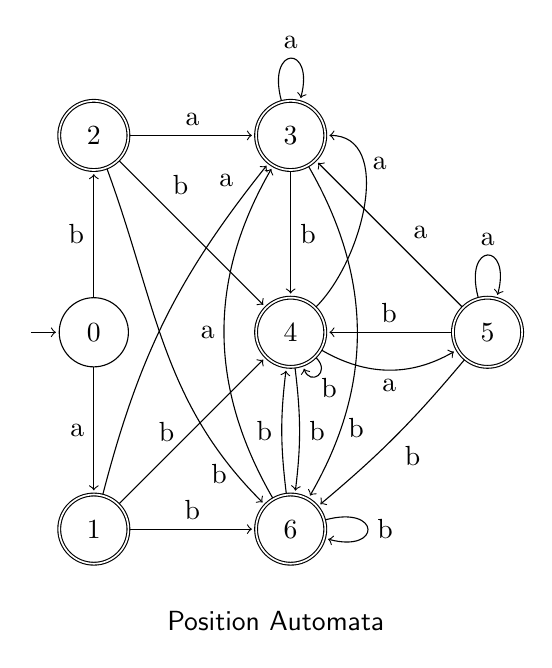
\begin{tikzpicture}[shorten >=1pt, node distance=2.5cm, on grid, auto]
        \tikzset{initial text={},initial where=left}
        % Define attributes for the initial node
        \tikzstyle{every initial by arrow}=[initial distance=1em,inner sep=0pt]

        \node[state,initial] (q_0) {$0$};
        \node[state,accepting] (q_1) [below=of q_0] {$1$};
        \node[state,accepting] (q_2) [above=of q_0] {$2$};
        \node[state,accepting] (q_3) [right=of q_2] {$3$};
        \node[state,accepting] (q_4) [right=of q_0] {$4$};
        \node[state,accepting] (q_5) [right=of q_4] {$5$};
        \node[state,accepting] (q_6) [right=of q_1] {$6$};
        \path[->]
        (q_0) edge node[left] {a} (q_1)
        (q_0) edge node {b} (q_2)

        (q_1) edge [bend left=12] node[pos=0.9] {a} (q_3)
        (q_1) edge node[pos=0.4,inner sep=1pt] {b} (q_4)
        (q_1) edge node {b} (q_6)

        (q_2) edge node {a} (q_3)
        (q_2) edge node[pos=0.3] {b} (q_4)
        (q_2) edge [bend right=5,in=200] node[left, pos=0.9] {b} (q_6)

        (q_3) edge [loop above] node {a} (q_3)
        (q_3) edge node {b} (q_4)
        (q_3) edge [bend left] node[pos=0.75,inner sep=1pt] {b} (q_6)

        (q_4) edge [out=45,in=360] node[right, pos=0.7] {a} (q_3)
        (q_4) edge [out=315,in=290,looseness=3.5] node[inner sep=1pt] {b} (q_4)
        (q_4) edge [bend right] node[below] {a} (q_5)
        (q_4) edge [bend left=7] node {b} (q_6)

        (q_5) edge node[pos=0.4,above right] {a} (q_3)
        (q_5) edge node[above] {b} (q_4)
        (q_5) edge [loop above] node {a} (q_5)
        (q_5) edge [bend left=5] node {b} (q_6)

        (q_6) edge [bend left] node {a} (q_3)
        (q_6) edge [bend left=7] node {b} (q_4)
        (q_6) edge [loop right] node {b} (q_6);

        \node[align=center,font=\sffamily,yshift=-2em] (title) at (current bounding box.south) {Position Automata};
    \end{tikzpicture}

    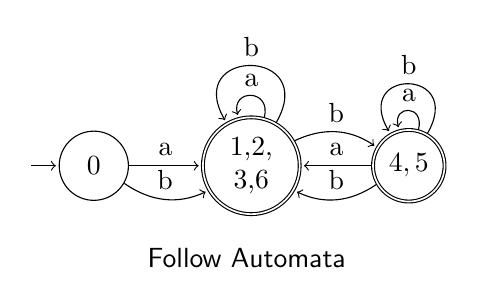
\begin{tikzpicture}[shorten >=1pt, node distance=2cm, on grid, auto]
        \tikzset{initial text={},initial where=left}
        % Define attributes for the initial node
        \tikzstyle{every initial by arrow}=[initial distance=1em,inner sep=0pt]

        \node[state,initial] (q_0) {$0$};
        \node[state,accepting,draw,align=center] (q_1) [right=of q_0] {1,2,\\3,6};
        \node[state,accepting] (q_2) [right=of q_1] {$4,5$};
        \path[->]
        (q_0) edge node {a} (q_1)
        (q_0) edge [bend right] node[above] {b} (q_1)

        (q_1) edge [out=75,in=105,looseness=3] node[above] {a} (q_1)
        (q_1) edge [out=60,in=120,looseness=4.5] node[above] {b} (q_1)
        (q_1) edge [bend left] node[above] {b} (q_2)

        (q_2) edge [out=75,in=105,looseness=3.5] node[above] {a} (q_2)
        (q_2) edge [out=60,in=120,looseness=5.25] node[above] {b} (q_2)
        (q_2) edge node[above] {a} (q_1)
        (q_2) edge [bend left] node[above] {b} (q_1);

        \node[align=center,font=\sffamily,yshift=-1.5em] (title) at (current bounding box.south) {Follow Automata};
    \end{tikzpicture}

\end{document}
